\section{Use-Case Modellierung für funktionale Anforderungen}
\label{sec:use-case-modellierung}

Nachfolgend wird die ursprüngliche Anwendung funktional Beschrieben, um daraus die Qualitätsanforderungen für die Migrierte Anwendung abzuleiten. Durch das Testen auf die Qualitätsanforderungen soll untersucht werden, ob sich eine Veränderung im Nutzungsverhalten bei der Migration in die Cloud ergibt.

\subsection{Funktionale Beschreibung der bisherigen Anwendung}
Die Funktionalität der bisherigen Anwendung besteht darin, den Prozess der Rechnungsstellung zu automatisieren und somit management Aufwände zu reduzieren. Dazu besteht die Anwendung hauptsächlich aus drei Services, dem \textit{Collect Service}, dem \textit{Check Service} und dem dem \textit{Report Service}. Ausgeführt wird die Anwendung bisher auf einem lokalen System und greift über das lokale Verzeichnis mithilfe einer \gls{Box}-Integration auf diese zu. Zur Ausführung der Anwendung wird eine Konfigurationsdatei benötigt, die alle notwendigen Pfade und Parameter enthält. In dem \gls{Box}-Verzeichnis liegen die \textit{\glspl{Timesheet}} der Mitarbeiter des Projektes und eine Projektmanagementdatei (PMO-File), die allgemeine Informationen zum Projekt und den Mitarbeitern enthält.

Aufgabe des \textit{Collect Service} ist es, aus dem PMO-File oder einer alternativen Mitarbeiterliste alle, aktuell in dem Projekt aktiven Mitarbeiter zu ermitteln und die \textit{\glspl{Timesheet}} dieser in ein \textit{Collect}-Verzeichnis zu kopieren. Der \textit{Check Service} gleicht die von den Mitarbeitern manuell ausgefüllten \textit{\glspl{Timesheet}} mit den Daten aus einem Zeiterfassungstool und ermittelt, ob die Daten korrekt sind oder gegebenenfalls korrigiert werden müssen. Abschließend werden im \textit{Report Service} aus den Daten die Rechnungen für den Kunden erstellt, indem die Informationen aus den \textit{\glspl{Timesheet}} detailliert auf die einzelnen Teilprojekten aufgeteilt und abgerechnet werden.

In dieser Arbeit soll untersucht werden, ob sich eine Veränderung im Nutzungsverhalten bei der Migration in die Cloud ergibt und ob die Business-Logik entsprechend angepasst werden muss. \pagebreak

\subsection{Wie könnte ein Cloud Setup Aussehen?}
Durch die Migration in die Cloud ergeben sich viele Möglichkeiten für die Anwendung. Unter anderem bringt die Cloud-Migration \textit{\gls{Multi-Tenancy}}, also eine Mehrbenutzerfähigkeit mit sich, damit die Anwendung von mehreren Nutzern gleichzeitig verwendet werden kann, ohne dass diese sich beeinflussen oder behindern.

Um die Anwendung allgemein in die Cloud zu migrieren, könnte diese so wie sie ist mit \textit{Lift-and-Shift} in eine virtuelle Maschine Kopiert werden und würde somit in der Cloud bereitgestellt. Dadurch könnte jedoch keine Aussage darüber getroffen werden, inwiefern die Anwendung oder ihre Architektur verändert werden muss, um die Vorteile einer Cloud-nativen Anwendung in der Cloud auszunutzen.

Aus diesem Grund soll die Anwendung zu einer Web-Anwendung weiterentwickelt werden. Dadurch verändert sich die Art und Weise, wie die Use-Cases Ausgeführt werden und wie die Anwendung benutzt wird. Diese Veränderungen werden am Beispiel der Migration des \textit{Collect Service} untersucht.

\subsection{Collect Service}
\textbf{Bisherige Verwendung:}

Der für den Prototypen ausgewählte Use-Case ist das ''Einsammeln'' der \textit{\glspl{Timesheet}}. Aus einer Konfigurationsdatei hinaus soll festgelegt werden für welches Projekt und welchen Zeitraum diese von dem Projektverzeichnis in ein temporäres Verzeichnis kopiert werden sollen. 

\textbf{Möglichkeiten einer Web-Anwendung:}

Durch die Migration in die Cloud und die Weiterentwicklung zu einer Web-Anwendung können die Funktionen der Anwendung zukünftig über einen API-Endpunkt bereitgestellt werden und die Ausführung dieser kann zum Beispiel nach einem Zeitplan oder einem Trigger, wie das Hochladen einer neuen Konfigurationsdatei erfolgen. Auf die hierzu notwendigen technischen Veränderungen wird später in der Arbeit eingegangen. \pagebreak

\textbf{Use-Case Definition:}

Nachfolgend wird der Use-Case definiert, um im Anschluss an die Implementierung untersuchen zu können, ob dieser auch nach der Migration in die Cloud erfüllbar ist.

\begin{figure}[H]
    \centering
    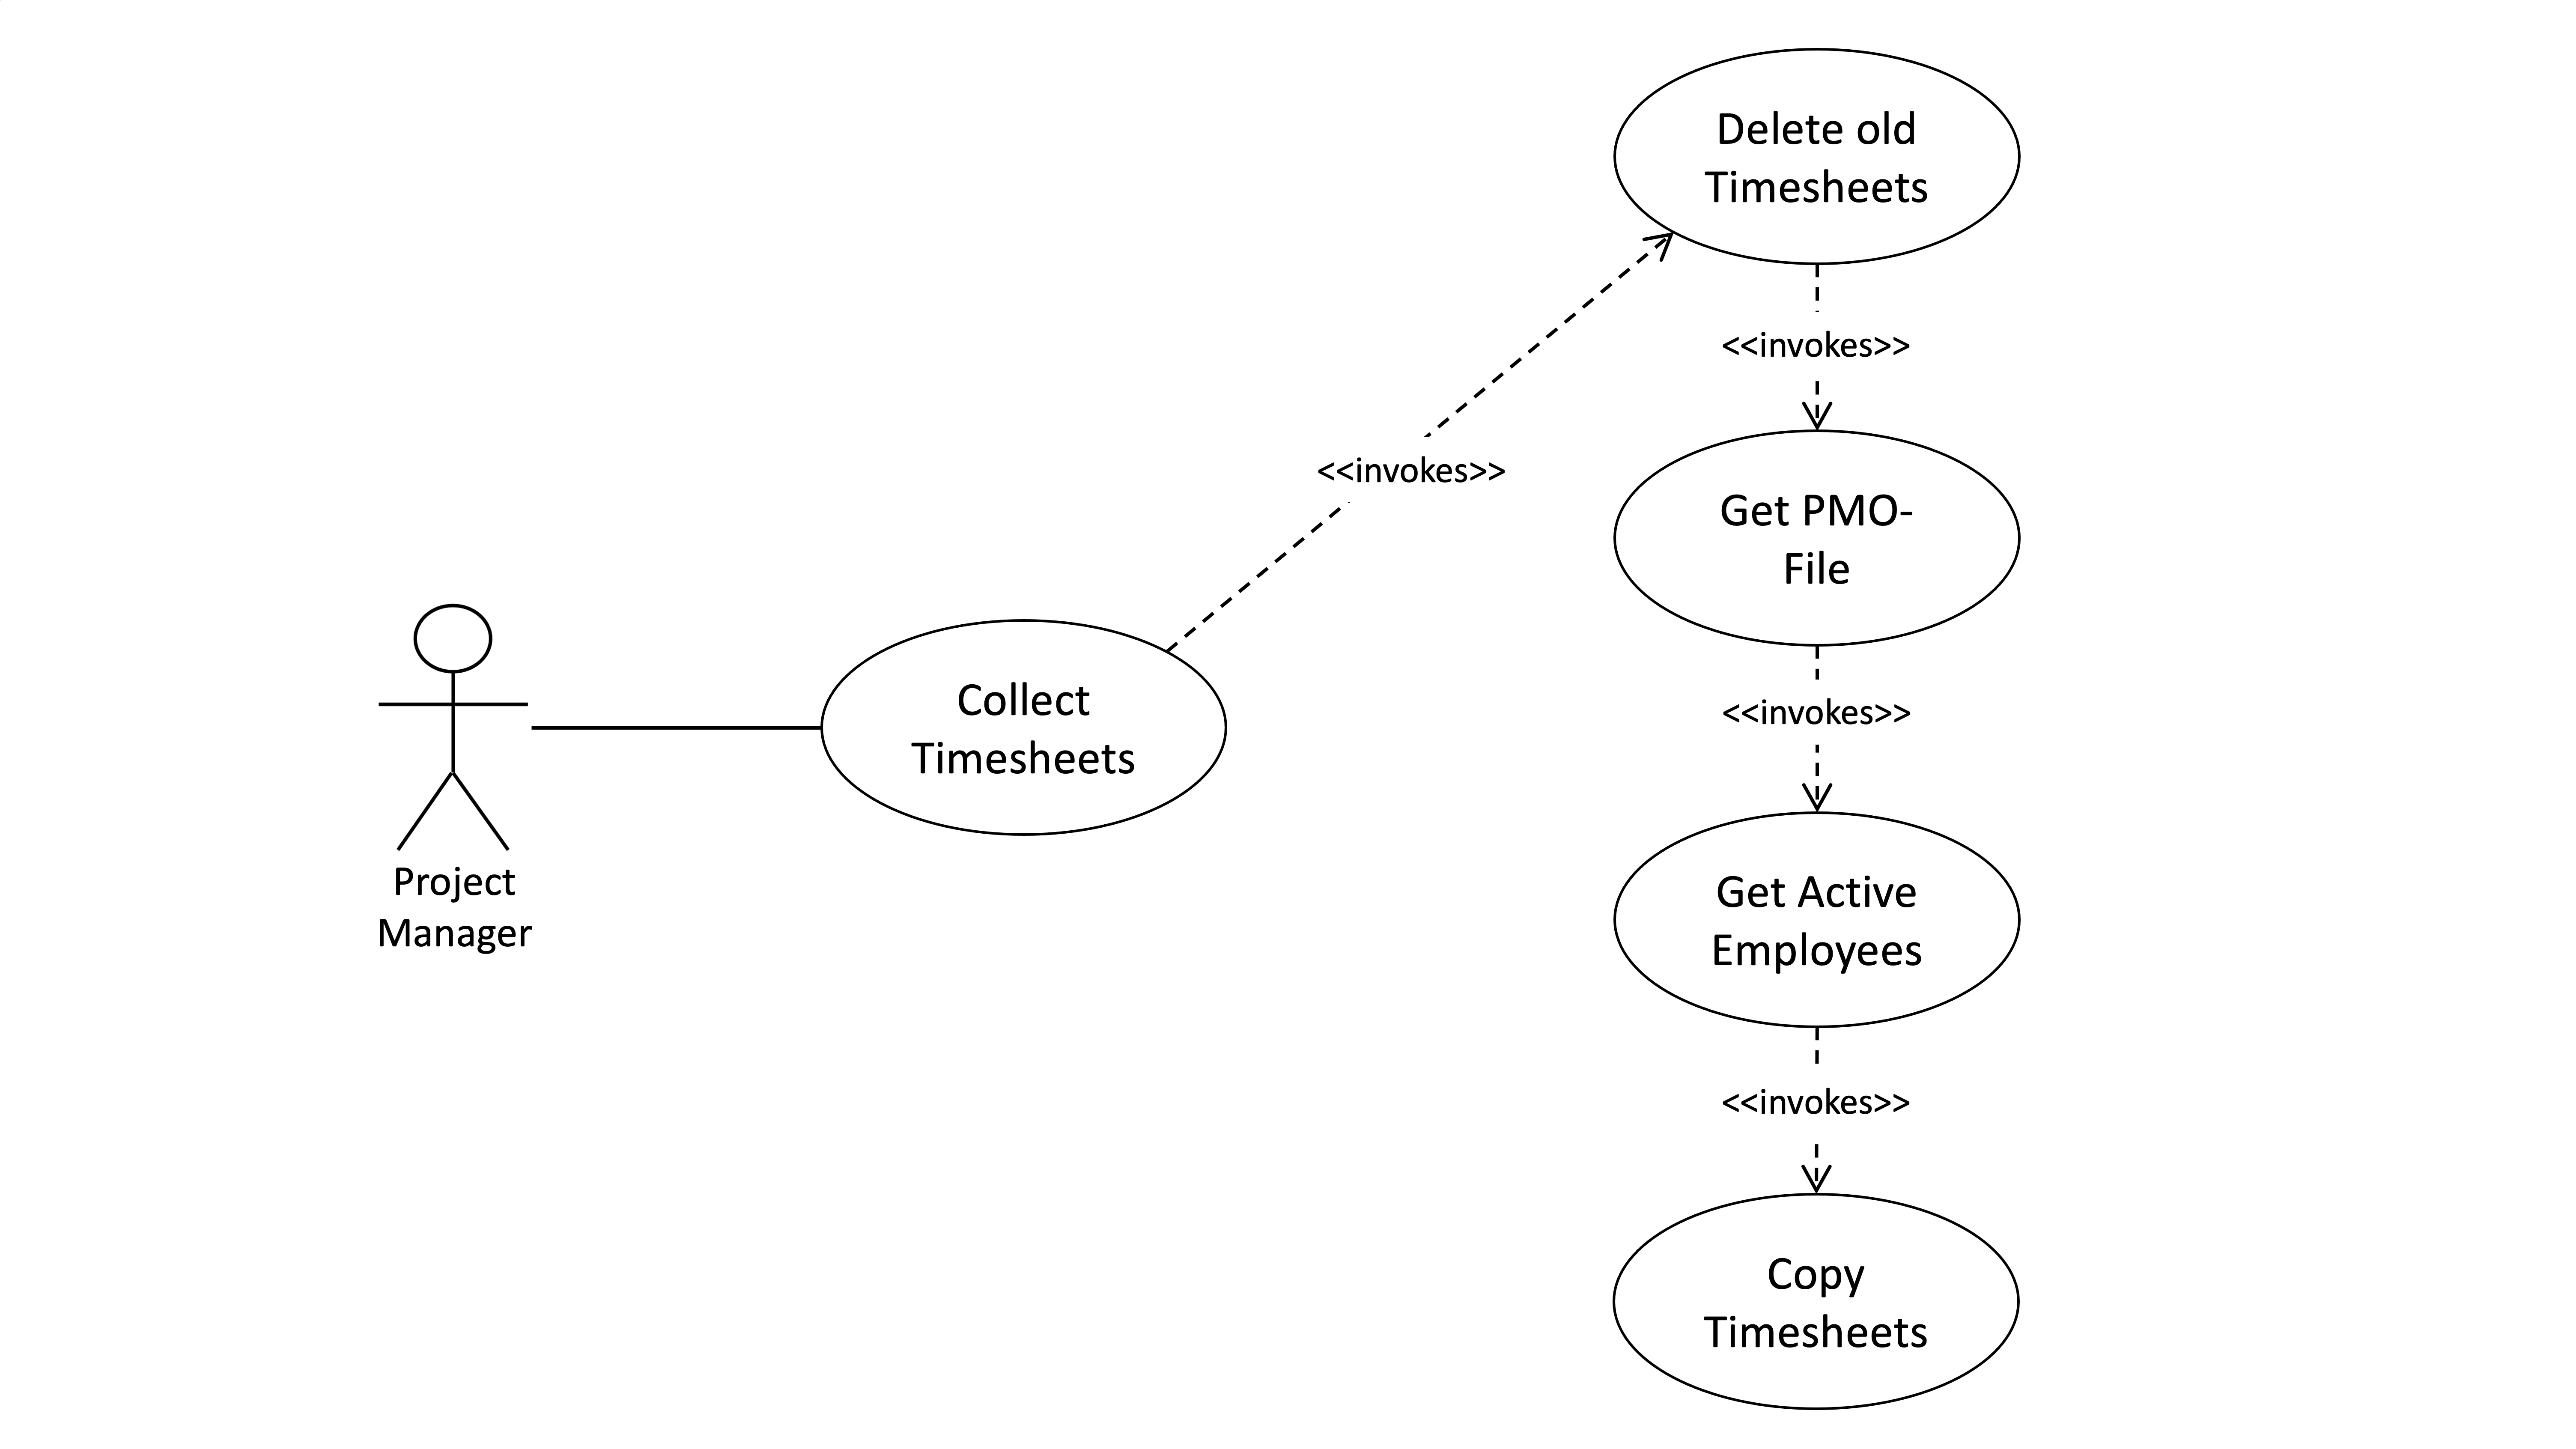
\includegraphics[width=\textwidth]{use-case-diagram.png}
    \caption{Use-Case Diagramm}
    \label{fig:use-case-diagram}
\end{figure}

Abbildung \ref{fig:use-case-diagram} stellt grafisch dar, welche Aufgaben der \textit{Collect Service} erfüllen muss und in welcher Reihenfolge diese ausgeführt werden. diese grundlegende Funktionsweise darf durch eine Cloud Migration nicht beeinträchtigt werden.

\begin{table}[H]
    \begin{tabular}[H]{|l|l|}
        \hline
        \multicolumn{2}{|l|}{\textbf{Anwendungsfall:} Einsammeln der \textit{\glspl{Timesheet}}} \\
        \hline
        \textbf{Kurzbeschreibung:} & \textit{\glspl{Timesheet}} aktiver Mitarbeiter in temporäres Verzeichnis kopieren \\
        \hline
        \multicolumn{2}{|l|}{\textbf{Normalverlauf}} \\
        \hline
        \multicolumn{2}{|l|}{1. Leeren des temporären Ordners} \\
        \multicolumn{2}{|l|}{2. PMO Datei finden und laden} \\
        \multicolumn{2}{|l|}{3. Aktive Mitarbeiter aus PMO Datei lesen} \\
        \multicolumn{2}{|l|}{4. \textit{\glspl{Timesheet}} der aktiven Mitarbeiter kopieren} \\
        \hline
        \multicolumn{2}{|l|}{\textbf{Alternativablauf}} \\
        \hline
        \multicolumn{2}{|l|}{Siehe Normalverlauf} \\
        \multicolumn{2}{|l|}{\textbf{Qualitätsanforderungen}} \\
        \hline
        \multicolumn{2}{|l|}{1. Für jeden aktiven Mitarbeiter soll ein \textit{\gls{Timesheet}}im temporären Ordner liegen} \\
        \multicolumn{2}{|l|}{2. Die \textit{\glspl{Timesheet}} sollen unverändert sein (Dateiname, Inhalt)} \\
        \multicolumn{2}{|l|}{3. Eigener Zielordner pro Monat zur Vermiedung von Vermischungen} \\
        \multicolumn{2}{|l|}{4. Die \textit{\gls{Timesheet}} Größe kann variieren -> keine Limitierungen} \\
        \multicolumn{2}{|l|}{5. Es darf keine Kompression mit Formatänderung eingesetz werden} \\
        \multicolumn{2}{|l|}{6. Ein Logfile soll Erfolg und Misserfolg von Kopiervorgängen enthalten} \\
        \multicolumn{2}{|l|}{7. Fehlersituationen auf einzelnen Dateien dürfen den Ablauf nicht unterbrechen} \\
        \multicolumn{2}{|l|}{8. Root-Verzeichnisse für Ziel und Quelle müssen konfigurierbar sein} \\
        \hline
    \end{tabular}
    \caption{Anwendungsfall: Einsammeln der \textit{\glspl{Timesheet}}}
    \label{tab:use-case-analyse-timesheets}
\end{table}

Anschließend an diesen Prozess würden die weiteren Services der Toolsuite folgen, die für den Umfang dieser Arbeit ausgelassen wurden.